% Fig 5:fig7 -- Distribucion del corpus por las 4 fuentes (pie chart TikZ).
% Porcentajes representativos del corpus electoral multifuente.
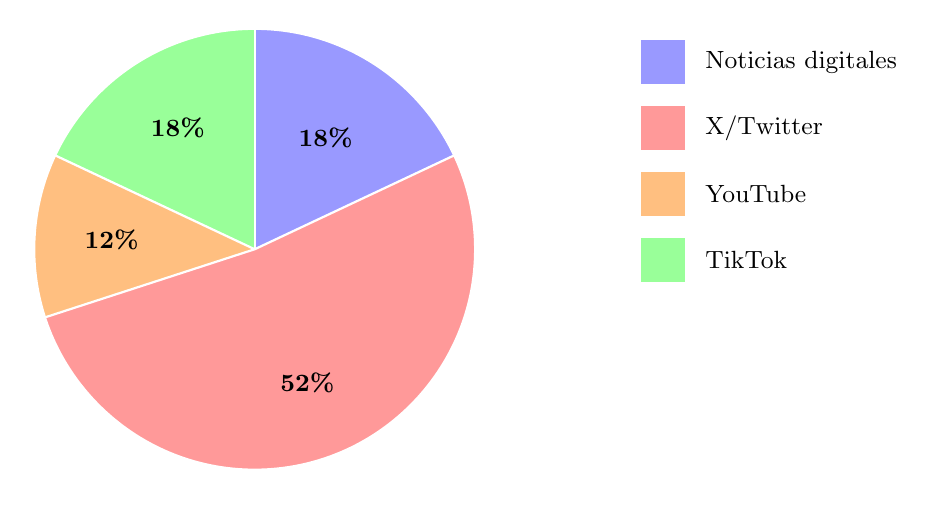
\begin{tikzpicture}[scale=1.4]
    % Datos: noticias 18%, X/Twitter 52%, YouTube 12%, TikTok 18%
    % Convertidos a angulos: 18%->64.8, 52%->187.2, 12%->43.2, 18%->64.8
    % Inicio en 90 grados (arriba), sentido horario
    \def\angA{90}      % inicio noticias
    \def\angB{25.2}    % fin noticias = 90 - 64.8
    \def\angC{-162}    % fin twitter = 25.2 - 187.2
    \def\angD{154.8}   % fin youtube = -162 - 43.2 -> 360 -> 154.8
    \def\angE{90}      % fin tiktok = vuelta completa

    % Sectores
    \fill[blue!40] (0,0) -- (\angA:2) arc (\angA:\angB:2) -- cycle;
    \fill[red!40]  (0,0) -- (\angB:2) arc (\angB:-162:2) -- cycle;
    \fill[orange!50] (0,0) -- (-162:2) arc (-162:-205.2:2) -- cycle;
    \fill[green!40] (0,0) -- (-205.2:2) arc (-205.2:-270:2) -- cycle;

    % Bordes
    \draw[thick, white] (0,0) circle (2);
    \foreach \a in {\angA,\angB,-162,-205.2} {
        \draw[thick, white] (0,0) -- (\a:2);
    }

    % Etiquetas con porcentajes
    \node[font=\small\bfseries] at (57.6:1.2)  {18\%};
    \node[font=\small\bfseries] at (-68.4:1.3) {52\%};
    \node[font=\small\bfseries] at (-183.6:1.3) {12\%};
    \node[font=\small\bfseries] at (-237.6:1.3) {18\%};

    % Leyenda
    \begin{scope}[shift={(3.5,1.5)}]
        \fill[blue!40]   (0,0)    rectangle (0.4,0.4);
        \fill[red!40]    (0,-0.6) rectangle (0.4,-0.2);
        \fill[orange!50] (0,-1.2) rectangle (0.4,-0.8);
        \fill[green!40]  (0,-1.8) rectangle (0.4,-1.4);
        \node[anchor=west, font=\small] at (0.5, 0.2)  {Noticias digitales};
        \node[anchor=west, font=\small] at (0.5,-0.4) {X/Twitter};
        \node[anchor=west, font=\small] at (0.5,-1.0) {YouTube};
        \node[anchor=west, font=\small] at (0.5,-1.6) {TikTok};
    \end{scope}
\end{tikzpicture}
